\documentclass{article}
\usepackage[utf8]{inputenc}
\usepackage{amsmath}
\usepackage{amsthm}
\usepackage{graphicx}
\usepackage{geometry}
\usepackage{caption}
\usepackage{hyperref}
\usepackage{minted}
\usemintedstyle{manni}
\geometry{a4paper, portrait, margin=1in}

\theoremstyle{plain}
\newtheorem{thm}{Theorem}

\theoremstyle{definition}
\newtheorem{defn}{Definition} % definition numbers are dependent on theorem numbers
\newtheorem{exmp}{Example} % same for example numbers

\hypersetup{
    colorlinks=true,
    urlcolor=blue,
}

\title{Operating Systems (UE18CS302)\\
    \large Unit 3}
\author{Aronya Baksy}
\date{August 2020}

\begin{document}
    \maketitle

\section{Introduction to memory management}
\subsection{Memory Protection}
\begin{itemize}
    \item All system memory is split into a hierarchy, with the differentiation being on the basis of speed, and capacity.
    
    \item The \textbf{CPU Cache} is closest to the CPU, has the greatest speed, but the smallest capacity. It is used to prevent CPU stalls while reading/writing to frequently used locations in the main memory.
    
    \item The presence of one (or many) fast caches in the CPU makes sure that the CPU does not have to wait unduly long time for memory access, as memory access is way slower than other CPU operations and can cause bottlenecks.
    
    \item Aside from speed, the concurrency and integrity of memory values stored must be maintained. User processes accessing memory must be protected from one another, and the OS kernel itself must be protected from all user processes. 
    
    \item The range of memory addresses that a single process is legally allowed to access is defined using a \textbf{base register} and a \textbf{limit register}.
    
    \item The base register holds the smallest memory address that the process can legally access, and the limit register holds the size of the range. The process can access every address in the range [base, base+limit] (both inclusive). 
    
    \item Every address generated by CPU in user mode is compared with this range, and if it falls outside the range then it leads to a \textbf{trap state} to the OS, that flags it as a memory access violation (fatal error). 
\end{itemize}

\begin{figure}[!h]
    \centering
    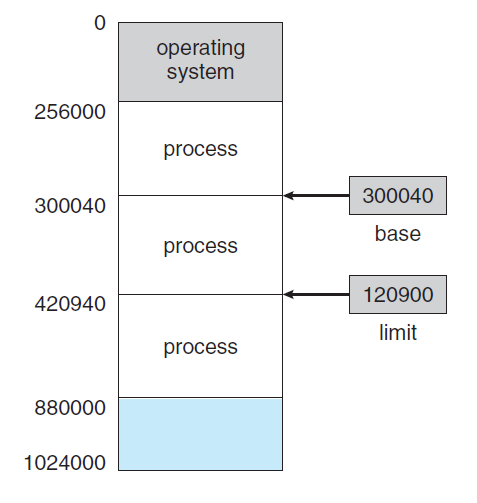
\includegraphics[scale=0.5]{os1.png}
    \caption{Base and Limit Register}
    \label{fig:my_label}
\end{figure}

\begin{figure}[!ht]
    \centering
    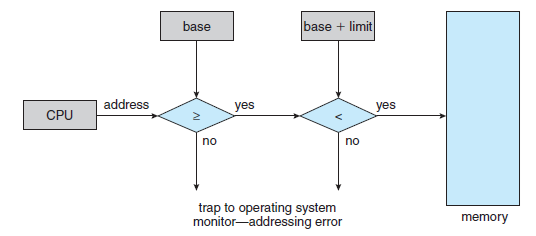
\includegraphics{os3.png}
    \caption{Address Protection using base and limit registers}
    \label{fig:my_label_1}
\end{figure}
\subsection{Address Binding}
\begin{itemize}
    \item Addresses in programs are represented \textit{symbolically} (using variable names and data types).
    
    \item The compiler \textbf{binds} these symbolic addresses to \textit{logical addresses} which are also known as relocatable addresses (eg: offset of 14 bytes from the beginning of this module).
    
    \item The linkage editor or the loader \textbf{binds} the logical addresses to \textit{physical addresses} (eg: offset of 14 bytes from module start gets bound to 70014).
    
    \item Each of these bindings are a mapping between 2 address spaces.
    
    \item The process of binding instructions and data to actual memory addresses can be done at:
    
    \begin{itemize}
        \item \textbf{Compile Time:} If the starting location of the process is known at compile time, then absolute addresses can be generated at compile time. If the starting address changes, then the program will have to be recompiled.
        
        \item \textbf{Load Time:} If the start address of the program is not known at compile time, then the compiler must generate relocatable (logical) addresses. These logical addresses can be bound to physical (ie. absolute) addresses when the program is loaded into the memory. If the starting address changes, then the program only has to be reloaded into the new address. 
        
        \item \textbf{Run Time} (Execution Time): If the process may be moved from one memory segment to another during its execution, then the binding must take place only at run time. This is the most commonly used method in modern OSes as it allows more efficient memory usage.
    \end{itemize}
\end{itemize}

\begin{figure}[!ht]
    \centering
    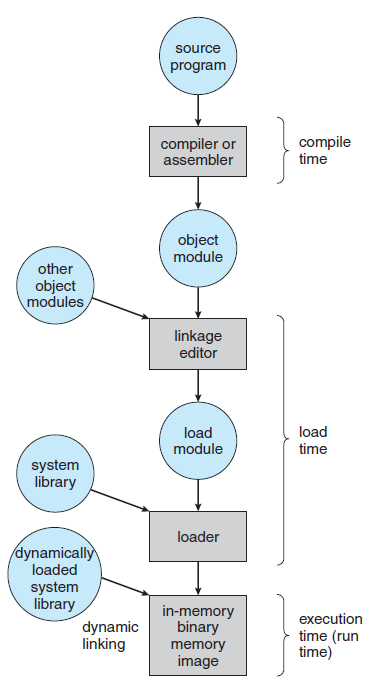
\includegraphics[scale = 0.6]{os2.png}
    \caption{User Program Processing}
    \label{fig:my_label_3}
\end{figure}

\subsection{Virtual and Physical Memory}
\begin{itemize}
    \item Addresses generated by CPU are referred to as \textbf{logical addresses}, while the address seen by the actual memory hardware (which is loaded into the \textbf{Memory Access Register} in the memory) is called the \textbf{physical address}. 
    
    \item In compile-time and load-time binding, the logical and physical addresses generated are identical. In run-time binding, the logical and physical address are different. 
    
    \item In compile time binding, the CPU generates the physical memory addresses directly, hence they are identical to the physical addresses in the memory. 
    
    \item In load-time binding, the relocatable addresses generated by the compiler are translated into physical addresses by the loader. Hence they are identical after loading to the physical addresses. 
    
    \item The run-time translation between logical (aka \textbf{virtual}) addresses and physical addresses is done by a hardware unit called the Memory Management Unit (MMU).
    
    \item All memory related computations (comparison with other addresses, arithmetic operations) are done on the virtual address, and the relocation (ie. translation between virtual and physical) is done only when a load or store is required. 
    
    \item The virtual address space has a range of (0, max) while the physical address space has a range of (R, R+max) where the base (ie. relocation) register holds the value of R.
\end{itemize}

\subsection{Dynamic Loading}
\begin{itemize}
    \item When an entire program sitting in the memory but some routines are only needed for a short time, it is inefficient in terms of memory usage.
    
    \item In dynamic loading, the routines are loaded from storage into the main memory only when they are called. 
    
    \item When the routine is loaded, the calling program's address table is updated and the relocatable addresses are translated into physical addresses, 
    
    \item Dynamic loading does not need support from the OS, it is the user programmer's responsibility to implement it. But libraries that implement some dynamic loading functionalities may be provided by the OS. 
\end{itemize}

\subsection{Dynamic Linking and Shared Libraries}
\begin{itemize}
    \item In dynamic linking, a system library that needs to be included in a user program is loaded only once, and all programs that use that library execute only one copy of it.
    
    \item Without dynamic linking, each user program would need its own copy of that system library which wastes memory space and disk space.
    
    \item The user program contains a \textbf{stub} which is a reference to the location of the dynamic library in the memory.
    
    \item When the stub is executed, it checks if the libary is already in memory. If not, it is loaded to memory, and if it is, then the stub replaces itself with the address of the routine and executes the routine. 
    
    \item If that library routine is referenced again, then it can be directly executed without any overheads of dynamic linking. 
    
    \item Shared libraries are a feature that enable several different versions of the same library to exist in memory, and the user program can choose which version to use. 
    
    \item Using shared libraries ensures that the majority of programs will not be affected by any change in versions of a library. 
    
    \item Dynamic linking and shared libraries require OS support, as only the OS can inspect the memory space of another process to see if a library exists in memory, and allow multiple processes to access that memory address. 
\end{itemize}

\section{Swapping}
\begin{itemize}
    \item Swapping is a mechanism that allows the total physical address space of all the processes in the system to exceed the main memory's address space, thus increasing the degree of multiprogramming.
    
    \item Swapping involves processes being moved between main memory and a \textbf{backing store}, then being brought back into main memory for continued execution.
\end{itemize}
\subsection{Standard Swapping}
\begin{itemize}
    \item The backing store in this case is a fast disk, that is large enough to store memory images for all users.
    
    \item A \textbf{ready queue} is used to store the processes that are in disk or memory that are ready to execute. 
    
    \item When the scheduler decides to run a process, it calls the dispatcher.
    
    \item The \textbf{dispatcher} checks if the next process to be executed lies in memory or not. If not, and there is not enough main memory space for the new process, the dispatcher swaps a process out of main memory and brings in the next process from the ready queue into the main memory.
    
    \item Knowing exactly the amount of memory that process is using (instead of what amount it \textit{might} use) is useful in reducing swap times (because swap time is proportional to the amount of memory being swapped). 
    
    \item Hence, a process that has changing memory requirements must notify the OS of these requirements using the system calls. 
    
    \item Only idle processes must be swapped, with special care on processes that have pending I/O.
    
    \item Solutions to swapping processes with pending I/O are:
    \begin{itemize}
        \item Don't swap out such processes
        
        \item Execute I/O ops only into the OS buffers. This means that there are 2 copies of the process (one in the OS buffer, one in the main memory). The transfer between these 2 happens only when process is swapped in again. This is known as \textbf{double buffering}. 
    \end{itemize}
    
    \item Standard swapping is not provided on modern OSes, but its variations are in use
    \begin{itemize}
        \item On UNIX, Linux and Windows, swapping is disabled by default until the free capacity in main memory falls below a certain amount. Swapping again stops when free capacity increases above another threshold.
        
        \item Swap only parts of processes instead of entire processes, to reduce swap time. 
    \end{itemize}
\end{itemize}

\subsection{Swapping on Mobile Systems}
\begin{itemize}
    \item Swapping is generally avoided in mobile systems as memory space is a more precious resource (because it is much rarer) than on desktop systems. 
    
    \item Other reasons to avoid swapping are the failure of flash memory (used in disk) beyond a certain number of writes, and the low throughput between flash and main memory.
    
    \item \textbf{iOS} asks applications to relinquish memory. Read only data is removed from main memory and reloaded later if needed. Modified data (like stack) is not removed from main memory, but any apps that fail to give up sufficient memory are terminated by the OS.
    
    \item \textbf{Android} follows a similar strategy to iOS, but the current application state is written to flash memory before it is terminated (for fast restart).
\end{itemize}

\section{Contiguous Memory Allocation}
\begin{itemize}
    \item Memory Allocation schemes aim to allocate memory to multiple user processes in memory at the same time in the most efficient manner. 
    
    \item In contiguous memory allocation, all the processes are assigned contiguous blocks of memory. 
\end{itemize}
\subsection{Allocation in CMA}
\begin{itemize}
    \item In \textbf{fixed partitioning}, the entire memory is divided into fixed size partitions where one process only can occupy one partition.
    
    \item The degree of multiprogramming is decided by the number of partitions
    
    \item Once a process terminates, that partition becomes available for another process, and the scheduler fills that partition from teh ready queue.
    
    \item In \textbf{variable partitioning}, the OS maintains a table of free and occupied partitions (available blocks of memory are referred to as \textit{holes}).
    
    \item The scheduler takes into account the memory requirement of the process while allocating memory. When the memory is allocated to the process, it runs until it terminates, and then the memory is freed.
    
    \item At any point in time, there is an input queue of processes, along with a list of free block sizes. 
    
    \item Memory is allocated until there is no hole large enough for the process at the front of the queue. 
    
    \item In this situation, the OS may wait until such a hole is available, or the OS may skip down the queue until a process is found that can fit in the currently available holes. 
    
    \item The scheduler needs to find holes that satisfy the memory requirement of the process. These holes may not be in any order, rather they are scattered throughout the memory randomly. 
    
    \item Holes can be managed in the following way: 
    
    \begin{itemize}
        \item If 2 adjacent holes end up becoming free, then they are merged into one larger hole.
        
        \item If a process ends up in a hole that is too large for it, the hole is split into two parts (one for the process, another free). 
    \end{itemize} 
    
    The table of free memory (ie. holes) and allocated memory needs to be updated any time this happens.
    
    \item The following strategies are used to select a hole from the available list of holes
    \begin{itemize}
        \item \textbf{First-Fit}: Select the first hole from the list of holes that is large enough for the incoming process.
        
        \item \textbf{Best-Fit}: Select the smallest hole that fits the incoming process. This requires searching the entire list of holes every time
        
        \item \textbf{Worst-Fit}: Allocate the largest hole that is currently in the list, to the incoming process. This also requires searching the entire list of holes every time.
    \end{itemize}
\end{itemize}

\subsection{Fragmentation}
\begin{itemize}
    \item \textbf{External Fragmentation} occurs when there are enough free holes to satisfy a process' requirements, but they are not contiguous hence the process must wait. 
    
    \item In the worst case, external fragmentation may result in a free hole between every two occupied blocks.
    
    \item Statistical analysis of the first-fit allocation shows that for every $N$ allocated blocks, $\frac{N}{2}$ blocks are lost to fragmentation. (loss of 33.33\%). 
    
    \item \textbf{Internal Fragmentation} occurs within partitions, when a process takes up memory that is smaller than the available hole size.
    
    \item eg: Let the partition size be 18464 bytes, and the process requests a block of size 18462 bytes. The free hole of size 2 bytes is inefficient to maintain (as its maintenance needs more overhead than 2 bytes). 
    
    \item The solution to the above is to allocate memory in fixed blocks, but this can result in slightly larger allocation than is needed. The difference between the used memory and the allocated block size is the extent of internal fragmentation.
    
    \item A solution to external fragmentation is called \textit{compaction}, where all the occupied memory blocks are compacted (ie. combined) together, and the holes all combine to become one large free hole. 
    
    \item Compaction will not work if address binding is done at compile time or linking time. But if address binding is done at run time, then compaction just means that the base register value needs to be changed once. 
    
    \item Another solution to fragmentation is to allow non-contiguous process memory spaces (ie. allow processes to take up non-contiguous memory blocks). The solutions that implement this are Segmentation and Paging.
\end{itemize}

\section{Segmentation}
\begin{itemize}
    \item The programmer's model of memory consists of blocks of variable sizes, each holding one specific functionality.
    
    \item Each \textit{segment} here defines either a method, a shared library, or some data structure (like stack, heap, objects etc.) with a base size and a length. 
    
    \item Individual elements inside the segment are referred to by their offset from the base address of that segment.
    
    \item Segmentation is a memory-management scheme that supports this programmer's model of memory.
    
    \item The logical address space is a collection of segments, each segment having a \textit{segment number} and a \textit{segment length}. 
    
    \item Every logical address consists of a tuple of $\langle$ segment\_number, offset $\rangle$ where the offset is the offset from the base address of the segment number.
\end{itemize}

\subsection{Hardware Support for Segmentation}
\begin{itemize}
    \item An address in the physical address space can be expressed from the programmer's point of view as the combination of the \textbf{segment number} $s$ and the \textbf{offset} within that segment $d$. 
    
    \item The \textbf{segment table} maps the 2-dimensional address $\langle$ s, d $\rangle$ to a single physical address. 
    
    \item The segment number $s$ is used as an index in the segment table.
    
    \item The CPU generated value of $d$ is compared with the value of $d$ from the segment table, and if the CPU generated value of $d$ is larger than the $d$ value from segment table, the system is sent into a trap state.
    
    \item If the CPU generated $d$ value is less than or equal to the $d$ value from the segment table, it is combined with the base address $s$ from the segment table to generate the physical address. 
\end{itemize}

\begin{figure}[!h]
    \centering
    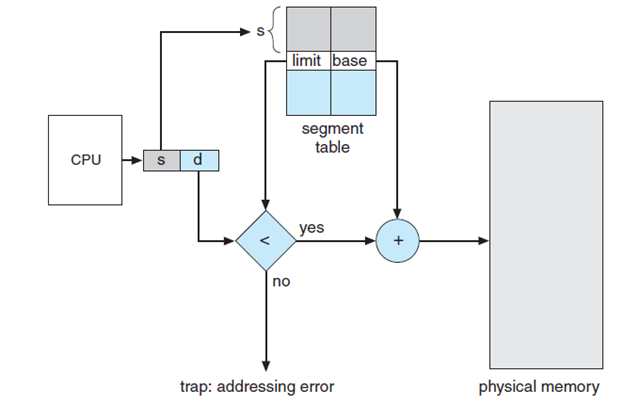
\includegraphics[scale=0.8]{os4.png}
    \caption{Hardware for Segmentation}
    \label{fig:my_label_4}
\end{figure}

\section{Paging}
\begin{itemize}
    \item Paging is another memory management technique that allows non-contiguous memory allocation, that avoid external fragmentation and the need for compaction (unlike segmentation).
    
    \item Physical memory is split into frames, and virtual memory is split into pages. Pages and frames have the same size.
    
    \item The logical address space is now totally separate from the physical address space, so a process can have a logical 64-bit address space even though the system has less than $2^{64}$ bytes of physical memory.
    
    \item The CPU generated virtual address consists of a \textbf{page number} $p$ and a \textbf{page offset} $d$. 
    
    \item The offset is carried over into the physical address as is. The page number is translated into the frame number $f$ by the \textbf{page table}. The page number is used to index in the page table, and the frame number is taken. 
    
    \item The combination of the frame number and the previously computed offset create a physical address. 
    
    \item Page and frame sizes are fixed by the OS as a power of 2. 
    
    \item If logical address space has size $2^m$, and page size is $2^n$, then the first $m-n$ bits of the logical address are the page number, and the last $n$ bits are the page offset. 
    
    \item Paging prevents external fragmentation but internal fragmentation still takes place in paging.
    
    \item Large page sizes cause larger extent of internal fragmentation, while smaller page sizes can cause greater overhead in the page table (as more entries will be needed which themselves take up memory). 
    
    \item Average page size in modern systems is 4-8 kB. 
    
    \item The \textbf{frame table} contains information about a frame of physical memory. Each physical page frame has one frame table entry.
    
    \item Each frame table entry stores whether the frame is free or allocated, and if allocated, the pid of the process that is occupying that frame. 
    
    \item The OS maintains a copy of the frame table for each active process. This copy is used when the user wants to make a system call referring to a particular address (this logical address must be translated into physical address using this copy of the page table).
    
    \item The process' copy of the page table is also referred to when the CPU dispatcher edits the hardware page table when the process is allocated the CPU. Therefore paging increases context switching time. 
\end{itemize}

\subsection{Hardware Support for Paging}
\begin{figure}[!h]
    \centering
    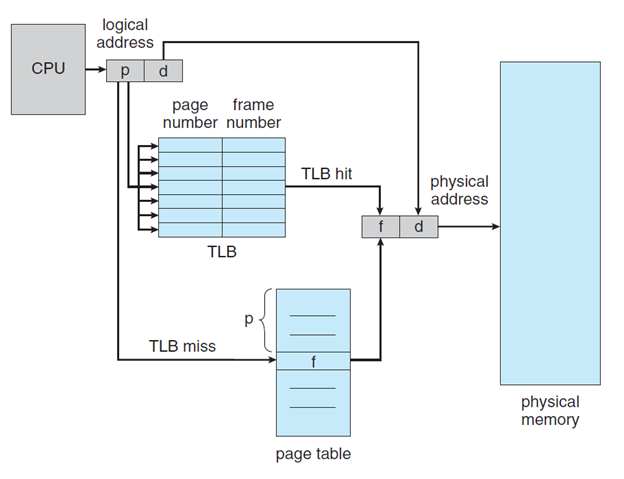
\includegraphics[scale=0.8]{os5.png}
    \caption{Paging Hardware}
    \label{fig:my_label_5}
\end{figure}
\begin{itemize}
    \item Page table can be implemented as a set of high speed CPU registers with fast logic for address translation. The CPU dispatcher loads and reloads the values in these registers. Instructions to modify the page table register values are privileged instructions.

    \item In modern systems with massive page tables (1 million+ entries), page tables are stored in main memory, and a \textbf{page table base register}(PTBR) denotes the start address of the page table. 
    
    \item The problem is that for a single address lookup, first the appropriate page table entry must be accessed (using PTBR + offset) and then the frame number in that page table entry must be accessed. Thus, for each memory access, two actual memory accesses are needed, which doubles the memory access time.
    
    \item The solution to the above is the use of a \textbf{translation look-aside buffer}(TLB), which acts like a high-speed cache for the page table. 
    
    \item The TLB entry consists of a key and a value. While searching, a key is simultaneously compared with all the keys in the TLB. 
    
    \item TLB searching is fast as it is part of the instruction pipeline. This means that the TLB must be of small size (between 32 and 1024 entries). 
    
    \item Some architectures use separate TLB for instruction and data addresses. 
    
    \item In case of a TLB miss, the address must be looked up in the memory (done either automatically by CPU or by an interrupt to the OS). The new page table entry must be placed into the TLB as well. 
    
    \item If the TLB is already full, then entries can be replaced using LRU or FIFO or random replacement. CPU or OS can participate in replacement (system dependent). 
    
    \item Some entries are \textbf{wired down} in the TLB, meaning they cannot be replaced. Typically kernel code addresses are wired down in the TLB. 
    
    \item In some TLBs, an ASID (\textbf{address space ID}) is stored in each entry. When the TLB tries to convert virtual address to a physical address, the ASID of the virtual page and that in the TLB entry are matched, and in case of a mismatch it is treated as a TLB miss. 
    
    \item The ASID offers address space protection, and allows the TLB to contain translation info for multiple processes at once. 
    
    \item If TLB does not support ASIDs, then everytime a new process is loaded onto the CPU the TLB must be entirely flushed as it might contain invalid translation info (valid virtual addresses but invalid physical addresses).
    
    \item The hit rate is defined as the probability of a TLB hit, ie. the chance that a particular request for a frame number will be satisfied by the TLB and not have to go all the way to the main memory page table. 
    
    \item The effective access time is defined as
    \begin{equation*}
        EAT = hit\text{ }rate \times a_h + (1-hit\text{ }rate)\times a_m
    \end{equation*}
    
    where $a_h$ and $a_m$ are the memory access times in case of a hit and a miss. 
    
    \item Assuming that TLB lookup requires one memory access, we can consider that $a_h$ is equal to the average memory access time (AMAT). And in case of a miss, two memory accesses are needed (one in the page table, another one for the actual memory byte), hence $a_m$ will be twice of the AMAT. 
    
    \item AMAT calculation is more complicated in case of multiple levels of TLBs (eg: Intel core i7 with 128 instruction entries and 64 data entries in Level 1 TLB, and 512 entries in Level 2 TLB). 
\end{itemize}

\subsection{Memory Protection}
\begin{itemize}
    \item Protection is implemented in page tables using separate bits associated with each page table entry. These bits are stored within the page table itself.
    
    \item These bits can be used to provide read-only, write-only and execute-only permissions, as well as various combinations of these. Illegal operations lead to a trap state within the OS.
    
    \item The \textbf{valid-invalid bit} is also attached to all the page table entries.  
    
    \item If the bit is set to \textit{valid}, then that page is a part of that process' logical address space, hence it can be accessed.
    
    \item If the bit is set to \textit{invalid}, that page is not a part of that process' logical address space, and any attempt to access it by that process will lead to a trap.
    
    \item The valid-invalid bit can cause problems if there is internal fragmentation, as a page table entry can be marked as valid even though the process only uses a few addresses within it and not the entire page. 
    
    \item A \textbf{page table length register}(PTLR) is maintained to check that the logical addresses generated by the CPU is in the valid range for that process. Failing this check leads to a trap. 
\end{itemize}

\subsection{Shared Pages}
\begin{itemize}
    \item Reentrant code (code that can be safely shared by multiple processes) can be placed into shared pages instead of having one copy per process, and it is non-self-modifying (ie. it does not change itself at run time, hence multiple processes can concurrently execute it). 
    \item The page table for each table refers to different pages for the process specific data, but the same pages are referred in all the tables for the reentrant code. 
    
    \item Heavily used programs like compilers, database systems, window mgmt systems etc. can be placed into shared pages. The OS enforces read-only protection instead of leaving it to the developer of that program. 
    
    \item Shared memory (used for IPC) is implemented using shared pages in some systems. 
    
    \item In the below example, the pages associated with a text editor \texttt{ed} are shared by 3 processes
\end{itemize} 

\begin{figure}[!h]
    \centering
    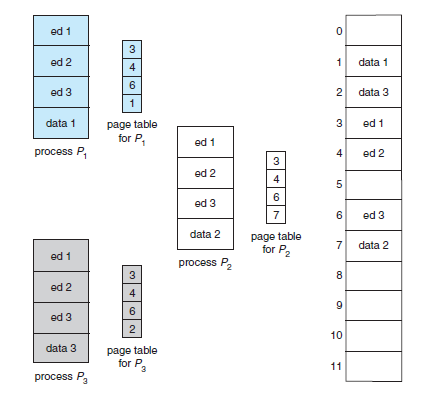
\includegraphics[scale=0.8]{os6.png}
    \caption{Shared Page Example}
    \label{fig:my_label_6}
\end{figure}

\section{Page Table Structure}
\subsection{Hierarchical Page Table}
\begin{itemize}
    \item In order to avoid large page table sizes the page table itself is split into pages. 
    
    \item The page number $p$ is split into a page table number $p_1$ and a page table offset $p_2$. 
    
    \item These 2 values are combined to get the frame number, and then that entry is combined with the page offset $d$ to get the physical location.
    
    \item eg: if virtual address space is of size $2^{32}$ and page is of size $2^{12}$ then in a single level page table there are $\frac{2^{32}}{2^{12}} = 2^{20}$ page table entries.
    
    \item If the 20 bit page number is split into 10 byte page table number and 10 byte page table offset, then the page table size is $2^{10} + 2^{10}$ which is smaller than the single level one. 
\end{itemize}
\begin{figure}[!ht]
    \centering
    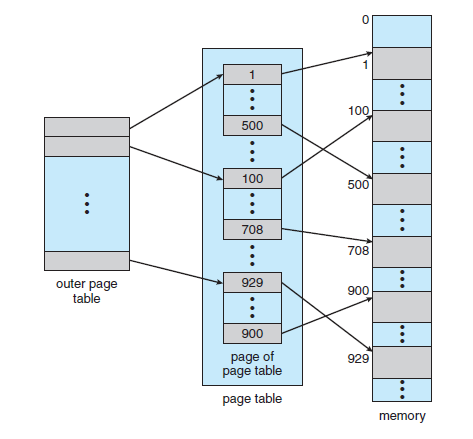
\includegraphics[scale=0.9]{os7.png}
    \caption{Hierarchical Page Table Structure}
    \label{fig:my_label_7}
\end{figure}

\begin{figure}[!ht]
    \centering
    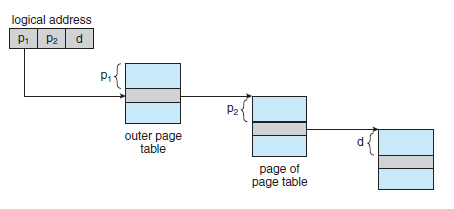
\includegraphics[scale=0.9]{os8.png}
    \caption{Address translation in Hierarchical Page Table}
    \label{fig:my_label_8}
\end{figure}

\begin{itemize}
    \item In the DEC VAX architecture (32 bit virtual memory addresses, 512 byte page size), the process' virtual memory is divided into 4 \textbf{sections} of size $2^{30}$ bytes each. 
    
    \item The first 2 bits (from left) of the virtual address are the section number, the next 21 are the page number and the last 9 are the page offset. 
    
    \item In the case where a process uses only one section, the page table is $2^{21}$ entries long, instead of $2^{23}$ without the use of hierarchical paging. For further reduction in page table size, each user process' page table is further paged.
    
    \item For 64-bit architectures, there is a tradeoff between large page table size (in case of 1 level page table) and prohibitive number of memory accesses (caused by too many levels of hierarchy). 
    
    \item A 32-10-10-12 page table split causes the outermost table to be $2^{32}$ entries long, which, if each entry is 4 bytes long, translates to 16 GB. 
\end{itemize}

\subsection{Hashed Page Table}
\begin{itemize}
    \item This is used to handle virtual address spaces larger than $2^{64}$ bytes.
    
    \item Each entry of the page table is a linked list of structures. Each element of the list contains: 1) The virtual page number, 2) The frame number corresponding to that page number and 3) pointer to next element in linked list.
    
    \item The index is determined by $hash\_fn(virtual\_page\_no)$. The linked list at that index is searched for the given virtual page number, and the appropriate frame number is pulled from the found node. 
    
    \item In a \textbf{clustered page table}, each entry of the hash table can contain frame numbers for several pages at a time (say 16 pages). 
    
    \item Clustered page tables are useful for sparse address spaces.
\end{itemize}

\subsection{Inverted Page Table}
\begin{itemize}
    \item To avoid large page table sizes, inverted page tables are used. 
    
    \item An inverted page table has \textbf{one entry per frame} of physical memory used. Each entry consists of the virtual address of the page that is using that physical location, and information about which process is using that frame (the PID or the ASID).
\end{itemize}
\begin{figure}[!h]
    \centering
    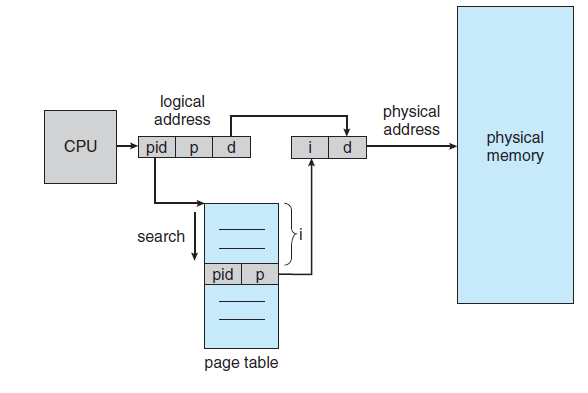
\includegraphics[scale=0.9]{os9.png}
    \caption{Inverted Page Table }
    \label{fig:my_label_9}
\end{figure}

\begin{itemize}
    \item The below example is for the IBM RT architecture. 
    
    \item Each virtual address consists of the tuple $\langle$ process id, page number, offset $\rangle$. 
    
    \item Each page table entry consists of the tuple $\langle$ process id, page number $\rangle$. The index $i$ of the page table is the physical address, that is transferred to the actual memory address along with the offset generated by CPU. 
    
    \item Searching takes time in inverted page tables because lookup happens through virtual address but the table is sorted in order of physical addresses. Hash tables are used to reduce lookup time but they cause an extra memory reference step. 
    
    \item Shared pages are hard to implement in inverted page tables, because shared pages mean that multiple virtual addresses (one per process that uses the shared page) map to the same physical address. A reference to a virtual address that is not mapped in the inverted page table will cause a page fault. 
\end{itemize}

\section{Demand Paging}
\begin{itemize}
    \item Instead of loading all the pages of a process into the memory at once, pages can be loaded only as and when \textbf{needed}. This is known as demand paging.
    
    \item Pages are loaded into memory only when the program requests them. 
    
    \item The \textbf{lazy swapper} (or pager, as it deals with swapping individual pages) brings in pages from disk into main memory only when they are requested, instead of bringing in all the pages associated with the process all at once.
    
    \item When a process is to be swapped in, the pager guesses which pages are to be brought in before the process is swapped out. 
    
    \item In order to distinguish the pages that are in disk and memory, the valid-invalid bit is used. If the bit is set to valid, then that page is a valid address for the process \textit{and} it is in memory. If it is invalid then either the page is an invalid address or it is a valid address but it is not in memory. 
    
    \item If the initial guess is correct then the process will run as if all pages were brought in, and no page faults occur.
    
    \item A \textbf{page fault} occurs when a process tries to access the address in a page that was not brought into the main memory. Such pages have entries in page table where they are marked \textit{invalid}. 
    
    \item An attempt to access such a page leads to a trap in the OS, and the trap is the result of the OS failing to bring in the desired pages. 
    
    \item Handling page faults in demand paging follows the below sequence of steps:
    \begin{enumerate}
        \item When a page fault occurs, the internal table (inside the PCB of that process) is checked to see if the reference was valid or not.
        
        \item If it was an invalid reference then the process is terminated.
        
        \item In case of a valid reference, the page that is not in main memory is paged in. First a free frame is located, a disk operation is scheduled to read the requested page into that located frame.
        
        \item Once the disk operation is done, the table inside the PCB and the page table are both updated to reflect this change. The instruction that was interrupted by the trap can now be restarted safely. 
    \end{enumerate}
    
    \item In \textbf{pure demand paging}, a process is started with \textbf{none} of its pages loaded in. One by one, the process goes through multiple page faults until all the required pages are in memory and the process can run to completion. 
    
    \item For each instruction that is executed, many pages can be accessed at the same time (a single instruction page and multiple data pages). The resulting number of page faults that pure demand paging would cause in this case would be unacceptable in terms of performance.
    
    \item Whenever page fault occurs, the current state of the currently executing instruction (registers, PC, condition code) must be saved so that the instruction can be restarted successfully. 
    
    \item This can be safely done for normal instructions that only modify one location at a time. The difficulty arises when instructions modify more than one location at a time (for example the \texttt{MVC} instruction in IBM System 360 architecture, that moves 256 bytes from one location to another (maybe overlapping) location). 
    
    \item If either source or destination straddles a page boundary, then page fault will occur in the middle of the instruction. If the source and dest overlap then the instruction cannot be restarted as the source may have been modified. 
    
    \item A simple solution to this is to have the instruction try to access both ends of both blocks before any moving of data. If any page fault is to happen, it will happen at this point, hence the original data is still safe and the instruction can be restarted. 
    
    \item Another solution is the use of temporary registers to store the old value that can be later written to the right location. In case of a page fault, the old values are overwritten into the original location and the instruction can be restarted. 
\end{itemize}

\subsection{Performance of Demand Paging}

\begin{itemize}
    \item The effective access time of demand paging is given by
    \begin{equation}
        EAT = (1-p)\times t_m + p\times t_{pf}
    \end{equation}
    Where $p$ is the probability of a page fault, $t_m$ is the average memory access time, and $t_{pf}$ is the time needed to service a page fault. 
    
    \item The page fault time $t_{pf}$ is the time needed to carry out the following steps:
    \begin{enumerate}
        \item Trap to the OS
        
        \item Save current process $P_1$ state, registers
        
        \item Check if access was legal or not. If it was legal then find location of that page on the disk. Allocate a disk read operation to a free frame.
        
        \item Wait for the disk read to take place. This includes the latency of the disk, and the transfer time from disk to memory.
        
        \item While the above is happening, allocate some other process $P_2$ to the CPU
        
        \item When disk read is done, an interrupt is received from the disk, and the currently running process $P_2$ is saved. If the interrupt is from the disk, then the page tables and process tables are updated. Wait for CPU to be allocated to $P_1$ again. 
        
        \item Restore the state of $P_1$ and resume the interrupted instruction.
    \end{enumerate}
    
    \item Demand paging is also affected by how the \textbf{swap space} is handled. As swap space is faster, it is better to load pages from swap space than from the actual file system. 
    
    \item One option is to load pages for the first time from the file system, but when they are replaced they are sent to the swap space. 
    
    \item Another option for binary files specifically, is to use the file system as a backing store, and when the page is to be replaced, it can just be overwritten in the same location in memory. For pages not associated with a file (like process stack/heap, aka \textbf{anonymous memory}), swap space has to be used. This approach is used on Solaris and BSD UNIX.
\end{itemize}

\section{Copy on Write}
\begin{itemize}
    \item This is an approach similar to shared pages, that is used when a child process is created using the \texttt{fork()} call in the parent. 
    
    \item The traditional approach is to make the child as an exact full copy of the parent address space. But since many child processes anyway erase the parent copy by using the \texttt{exec()} call, this copying is not necessary. 
    
    \item In copy on write, initially the child and parent share the same pages, and these pages are marked as Copy on write pages. 
    
    \item If one of the process wishes to modify such a page, then the OS creates a copy of the page, maps it to that process address space, and then allocates that page to the process that modified. 
    
    \item Only pages that can be modified are marked as CoW. Non modifiable pages (like code) are still shared by parent and child. 
    
    \item Free pages are allocated to the process that modifies, from a \textbf{pool} of free pages. This pool of free pages is used when stack/heap for a process has to expand, or CoW needs to take place. 
    
    \item OSes uses \textbf{zero fill on demand} pages that have been filled with 0 before allocating (to clear out the previous content). 
    
    \item The \texttt{vfork()} system call in UNIX is used to create a new process without creating a copy of the parent process' memory. The child shares all memory with parent until it issues an \texttt{exec()} call, then the copy is done and the appropriate code is loaded onto the process memory.
    
    \item As \texttt{vfork()} uses CoW, it must be used with caution so that the child does not modify the parent's address space. It is intended to be used when child calls \texttt{exec()} immediately after creation. 
\end{itemize}

\section{Page Replacement}

\begin{itemize}
    \item Page replacement is used to handle the case when there are no free frames in the memory, but a new page is to be loaded from the disk. 
    
    \item With page replacement, the sequence of steps in handling a page fault changes to:
    \begin{enumerate}
        \item When a page fault occurs, the internal table (inside the PCB of that process) is checked to see if the reference was valid or not.
        
        \item If it was an invalid reference then the process is terminated.
        
        \item In case of a valid reference, the page that is not in main memory is paged in. If a free frame is found, then it is used. If no free frame is found, a page-replacement algorithm selects a \textbf{victim frame}. The victim frame is swapped out and the new page is loaded in its place.
        
        \item Once the disk operation is done, the table inside the PCB and the page table are both updated to reflect this change. The instruction that was interrupted by the trap can now be restarted safely. 
    \end{enumerate}
\end{itemize}

\begin{figure}[!h]
    \centering
    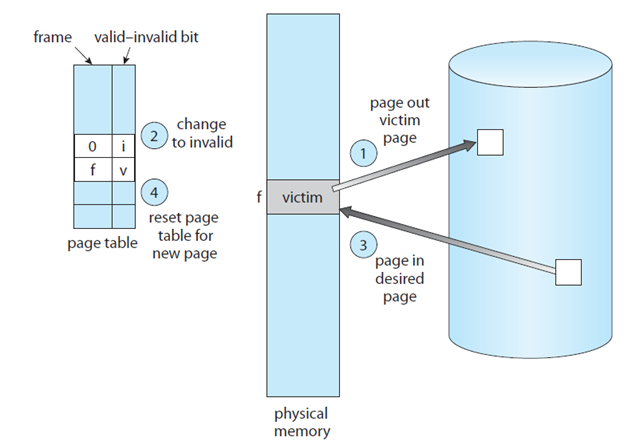
\includegraphics[scale=0.8]{os10.png}
    \caption{Page Replacement }
    \label{fig:my_label_10}
\end{figure}

\begin{itemize}
    \item Every time page replacement takes place, there are 2 disk operations that take place. This doubles the page fault service time $t_{pf}$ in case replacement must take place. 
    
    \item The number of disk operations involved in page replacement can be reduced by the use of a \textbf{modify bit} (or a \textit{dirty bit}) in the page table.
    
    \item If the modify bit is set, then the page has been modified since it was loaded from disk, and if the bit is not set then it is not modified since it was loaded from the disk.
    
    \item If the modify bit of a victim page is not set, then it does not have to be written back to the disk (the new page can simply overwrite on the existing page). 
    
    \item Page replacement (along with demand paging) is the crucial link between virtual and physical memory. 
    
    \item eg: If a process needs 20 pages to run, then without demand paging all 20 pages must be in the physical memory. But with demand paging, the process can take up only 10 pages and the rest of the pages can be loaded only when they are needed using some page replacement algorithm.
    
    \item This means that a larger virtual memory space can be given to the process, while the actual physical memory size is still the same. 
    
    \item The components of the paging system are a \textbf{frame-allocation} algorithm (with multiple processes in memory, how many frames does each one get) and a \textbf{page replacement} algorithm (if no free frame is available, which frame is selected as victim and swapped out of memory).
    
    \item Performance of page replacement algos is tested on a reference string of address (which can be converted into a reference string of page numbers) and a fixed number of frames, and counting the number of page faults. Less page faults mean better performance.
\end{itemize}

\subsection{FIFO Page Replacement}
\begin{itemize}
    \item Out of all pages in the memory, the page that was bought in first is swapped out.
    
    \item The below example considers a memory of size 3 frames. 
\end{itemize}
\begin{figure}[!h]
    \centering
    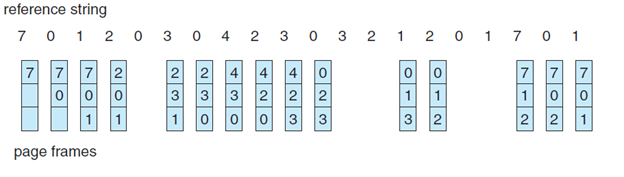
\includegraphics[scale=0.8]{os11.png}
    \caption{FIFO Page Replacement}
    \label{fig:my_label_11}
\end{figure}
\begin{itemize}
    \item FIFO is simple and easy to implement, but causes sub-optimal performance (if the oldest page happens to be one that is constantly in use, then replacing it can cause immediate page fault and one more replacement).
    
    \item FIFO also suffers from \textbf{Belady's Anomaly}, which is an experimental result. The observation is that increasing the number of frames in memory does not reduce the number of page faults. 
\end{itemize}

\subsection{Optimal Page Replacement Algorithm (OPT)}
\begin{itemize}
    \item The page that \textit{will not be used} for the longest time is replaced. 
\end{itemize}
\begin{figure}[!h]
    \centering
    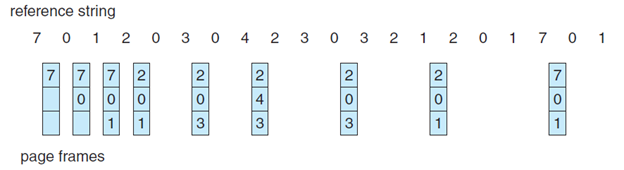
\includegraphics[scale=0.8]{os12.png}
    \caption{Optimal Page Replacement}
    \label{fig:my_label_12}
\end{figure}

\begin{itemize}
    \item OPT offers excellent performance (better than FIFO) but is hard to implement as it requires future knowledge of what pages be used in the reference string. 
    
    \item OPT also does not suffer from Belady's Anomaly
\end{itemize}

\subsection{LRU Page Replacement}
\begin{itemize}
    \item The page that \textit{has not been used} for the longest time is replaced.
\end{itemize}
\begin{figure}[!h]
    \centering
    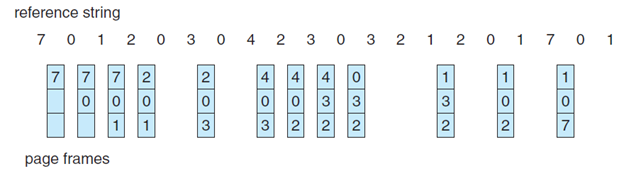
\includegraphics[scale=0.8]{os13.png}
    \caption{LRU Page Replacement}
    \label{fig:my_label_13}
\end{figure}

\begin{itemize}
    \item LRU is the exact reverse logic of OPT algorithm. 
    
    \item Let $S$ be  a reference string and $S^r$ be the reverse of $S$. The page fault rate on a s$S$ using LRU would be the same as the page fault rate $S^r$ using OPT.
    
    \item LRU can be implemented using
    \begin{itemize}
        \item \textbf{Counters}: 
        \begin{enumerate}
            \item Every page table entry has a time-of-use field and there is a single clock register attached to it.
            
            \item  Whenever a reference is made to a page, the time of use field of that page table entry is assigned the current clock register value. 
            
            \item For every page replacement, the entire page table is searched and the page with the smallest time value is replaced.
            
            \item Clock overflow, changes to page table (because of scheduling) and the number of memory writes (one for changing time of use in the page table) are to be considered.
        \end{enumerate}
        
        \item \textbf{Stack}:
        \begin{enumerate}
            \item A stack of page numbers is maintained. 
            
            \item Whenever a page is referenced, it is removed from the stack and put on the top. In this way, the most recently used page is always at the top of the stack and the least recently used page is always at the bottom
            
            \item Since page must be removed from the middle of the stack, the stack is implemented as a doubly-linked list, with a head and a tail pointer
            
            \item Every update to the stack requires changing at most 6 pointers and getting the LRU page is easy (tail pointer). 
        \end{enumerate}
    \end{itemize}
\end{itemize}

\section{Frame Allocation}
\begin{itemize}
    \item The simplest strategy for frame allocation is to put all the free frames in memory in the free-frame list, and all processes can share from this pool.
    
    \item The OS can also be allowed to use the free frames for buffers and tables, but a certain number of frames are always reserved as free frames, so that if replacement must happen, then a free frame is always available. 
\end{itemize}

\subsection{Minimum Number of Frames}
\begin{itemize}
    \item Every process must be allocated a certain minimum number of frames when it is loaded. This is primarily done for performance reasons, so that memory references do not result in page faults.
    
    \item If there are $n$ levels of possible memory references, then $n+1$ pages must be loaded into the memory at minimum. 
    
    \item The number of levels of indirection must be restricted to ensure that the physical memory is not filled up entirely by one process' pages. 
    
    \item The maximum number of frames is dictated by the amount of physical memory, and the miniumum number of frames is defined by the architecture (the number of indirect references dictates this). 
\end{itemize}

\subsection{Allocation Algorithms}
\begin{itemize}
    \item In \textbf{equal allocation}, the $m$ available frames are distributed among the $n$ processes in equal proportion. Each process gets $m/n$ frames of memory. 
    
    \item This results in unused memory if the number of frames allocated is too large for the process size.
    
    \item In \textbf{proportional allocation}, each process is allocated frames according to its size. If the size of process $p_i$ is $s_i$, then the total size of all the processes is
    \begin{equation*}
        S = \sum_{i=1}^{n} s_i
    \end{equation*}
    and the allocation for each process is
    \begin{equation*}
        a_i = \frac{s_i}{S} \times m
    \end{equation*}
    where $m$ is the total number of available frames. $a_i$ is rounded up to the nearest integer so that it is greater than the minimum number of frames needed per process according to the architecture. 
    
    \item Allocation varies according to the degree of multiprogramming in the system. In case of increased multiprogramming, processes will lose some frames to accommodate new processes that enter the system. 
    
    \item Both equal and proportional allocation treat high priority processes and low priority processes as equals. The proportional allocation scheme can be modified to use priorities of processes instead of their relative size. 
\end{itemize}

\subsection{Global v Local Allocation}
\begin{itemize}
    \item All page replacement algorithms can be classified into global (victim frame is selected from the entire memory) and local (victim frame is selected from frames that are allocated only to that process).
    
    \item In a priority-based global allocation system, the high priority processes can select frames that are allocated to lower priority processes for replacement. But in this scheme a process does not have full control on its page fault rate as other processes are also involved in selecting frames for replacement.
    
    \item In local allocation however, the process' own less used pages are not available to it, hence causing lower system throughput. Hence global allocation is preferred.
\end{itemize}

\subsection{UMA vs NUMA}
\begin{itemize}
    \item Memory access on NUMA systems can depend on whether the memory to be accessed is on the same board as the CPU who is accessing it, or on a different board. 
    
    \item Allocation algorithms that take NUMA into account offer better performance on NUMA systems compared to algorithms that do not. 
    
    \item The algorithmic changes consist of having the scheduler track the last CPU on which each process ran. If the scheduler tries to schedule each process onto its previous CPU, and the memory-management system tries to allocate frames for the process close to the CPU on which it is being scheduled, then improved cache hits and decreased memory access times will result.
    
    \item A process with many \textit{threads} can end up with those threads scheduled on different boards. 
    
    \item In Solaris, there are \textbf{lgroups} (Latency groups) of CPU and memory that are close to each other. The scheduler tries to schedule all the threads of a process within the same (or nearest) lgroup and allocation happens within that lgroup. 

\end{itemize}

\section{Thrashing}
\begin{itemize}
    \item A process is said to be thrashing if it spends more time on paging activities (like page replacement) than on actual execution. 
    
    \item Given any process that does not have enough pages, and all of the pages are in active use. A page fault occurs and one of the currently active pages is replaced, which causes another page fault. This causes a never ending sequence of page faults.
\end{itemize}

\subsection{Cause of Thrashing}
\begin{itemize}
    \item If the CPU utilization falls below a certain extent, the OS loads new processes into memory. 
    
    \item Considering a global allocation system, the processes replace frames without regard for which process they belong to. Thus the processes that lose frames start to encounter page faults, thus selecting frames from other processes to be replaced, causing those processes to encounter page faults, and so on. 
    
    \item As more and more page faults occur, more and more page in requests are made to the disk, thus processes wait for the disk in a queue. While they wait, no work is being done, hence the CPU utilization falls and the OS loads in more processes.
    
    \item As these processes wait for paging to occur, throughput of the system falls, and \textbf{thrashing} starts. 
\end{itemize}
\begin{figure}[!h]
    \centering
    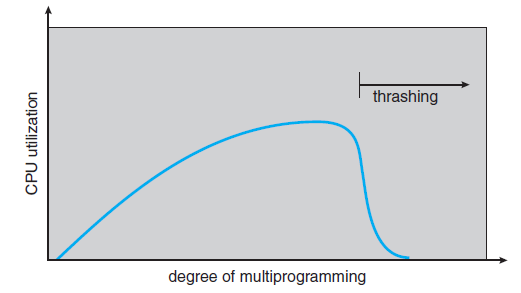
\includegraphics{os14.png}
    \caption{Thrashing}
    \label{fig:my_label_14}
\end{figure}
\begin{itemize}
    \item The effects of thrashing can be limited using a \textbf{local replacement} or a \textbf{priority replacement} algorithm. 
    
    \item With local replacement, one process that is thrashing cannot cause cause other processes to thrash by stealing their frames and replacing them. 
    
    \item But if a process is thrashing, it occupies its place on the disk queue indefinitely, hence the average page fault service $t_{pf}$ increases even for processes that are not thrashing.
    
    \item The locality assumption is used to develop the \textbf{working-set model} that is used to solve this issue.
    
    \item The assumption of locality states that a process uses a group of pages that are active all at once (this group is called a locality, and multiple localities can be overlapping), and processes can move between localities. 
    
    \item Caching is another technique that makes use of the principle of locality. 
    
    \item If all the frames are allocated for one locality, then the process will first fault until all the pages of that locality are loaded in memory, and then it will not fault until it switches localities. 
    
    \item If frames are allocated less than the process' locality size, then it will thrash as all the pages it is actively using cannot fit in memory.
\end{itemize}

\subsection{Working Set Model}
\begin{itemize}
    \item A parameter $\Delta$, called the \textit{working-set window} is used in this model. The set of $\Delta$ most recently used pages is the working set. 
    
    \item The current working set at time t is the set of $\Delta$ most recent pages that were referenced before that time t. The working set can be thought of as an estimate to the locality of the process.
    
    \item The accuracy of the working set depends on the value of $\Delta$. If it is too small then it will not cover the entire locality, and if it is too large then it overlaps many localities. 
    
    \item The total page demand $D$ is calculated as 
    \begin{equation*}
        D = \sum_{i=1}^{n} WSS_i
    \end{equation*}
    
    \item If $D>m$ then thrashing will occur as the demand is more than the number of free frames. 
    
    \item The OS monitors the working set of each process, and allocates as many frames as the working set size to that process. If enough extra frames are available then another process can be initiated. 
    
    \item If the sum of the working-set sizes increases, exceeding the total number of available frames, the operating system selects a process to suspend. The process’s pages are written out (swapped), and its frames are reallocated to other processes. The suspended process can be restarted later.
    
    \item The working-set model can be approximated with a fixed-interval timer interrupt and a reference bit. 
    
    \item For example, let $\Delta$ equals 10,000 references and that timer interrupt occurs every 5,000 references. 
    
    \item When a timer interrupt happens, the reference bit values are copied and cleared for each page. Thus, if a page fault occurs, the current reference bit and two in-memory bits can be examined to determine whether a page was used within the last 10,000 to 15,000 references. 
    \item If it was used, at least one of these bits will be on. If it has not been used, these bits will be off. Pages with at least one bit on will be considered to be in the working set.
\end{itemize}

\subsection{Page Fault Frequency Model}
\begin{itemize}
    \item Thrashing leads to an increase in the page fault rate, and the PFF model is a method to control the page fault rate. 
    
    \item Thresholds are set for max and min page fault rate. If the page fault rate exceeds the upper bound, then more frames are allocated to that process. If page fault rate falls below the lower bound, a frame is removed from that process address space.
    
    \item If the page-fault rate increases and no free frames are available, a process must be selected and swapped out to backing store. The freed frames are then distributed to processes with high page-fault rates
\end{itemize}

\section{Case Studies in Memory Management}
\subsection{Intel IA-32 Architecture}

\subsubsection{Segmentation Hardware}
    \begin{itemize}
        \item There are 16K segments per process, and each segment is allowed to be as large as 4 GB.
        
        \item The logical memory of a process consists of these 16K segments divided into two partitions. One partition is private only to that process, and its segment table is called the \textbf{Local Descriptor Table} (LDT). The other one is meant to be shared between all processes, and its segment table is called the \textbf{Global Descriptor Table} (GDT).
        
        \item Each entry in the LDT and GDT is 64 bits long, with detailed info about that segment. 
        
        \item The \textit{selector} is a 16 bit portion of the table entry that consists of a 13-bit segment number, one bit that indicates GDT or LDT, and 2 protection bits. The offset is a 32-bit number that specifies the location of the byte within the segment. 
        
        \item The machine has 6 segment registers (allowing six segments to be addressed at any one time by a process), and 6 microprogram registers to hold the corresponding descriptors from either the LDT or GDT. This cache lets the processor avoid having to read the descriptor from memory for every memory reference.
        
        \item The segment register points to the appropriate entry in the LDT/GDT, and the base+limit info from the descriptor is used to generate a 32-bit linear address. 
    \end{itemize}

\subsubsection{Paging Hardware}
    \begin{itemize}
        \item Intel IA-32 architecture supports page sizes of 4KB or 4 MB.
        
        \item For 4KB pages, a 2-level hierarchical page table is used. The 32 bit virtual address generated above is converted into a 10, 10, 12 bit split. The first 2 groups of 10 bits are the page numbers in the lower level of the page table, and the last 12 bits are the page offset. 
        
        \item The outermost level of the page table hierarchy is called the \textbf{page directory}.
        
        \item For 4MB pages, the leftmost 10 bits are the page number and the remaining 22 bits are the page offset. The middle level of the hierarchy is bypassed altogether. 
        
        \item The page size is mentioned in the \texttt{Page\_Size} field of the page directory. (1 for 4MB, 0 for 4KB).
        
        \item The page tables can be swapped to and from disk. The page directory maintains a valid-invalid bit to check if the inner page table referred to is in memory or not. 
        
        \item Under the \textbf{page-address extension}(PAE) scheme, the two level hierarchy is split into 3 levels, and the page-directory and page-table entries are now 64 bits long (instead of 32 without PAE). 
        
        \item Now the base address of page tables and page frames is expanded to 24 bits (instead of 20) and this combined with the 12-bit offset leads to a total of $2^{36}$ bits or 64GB of total addressable memory. 
        
        \item With the three level hierarchy, page sizes supported are 4 kB and 2 MB. 
    \end{itemize}
    
\subsubsection{Intel x64 architecture}
\begin{itemize}
    \item Instead of using all 64 bytes for memory addressing, only 48 bytes are used to address.
    
    \item 4 levels of paging hierarchy provide support for page sizes of 4kB, 2MB or 1 GB. 
    
    \item Due to the use of PAE, the 48 byte address can be used to address $2^{52}$ bytes or 4096 TB of physical memory. 
\end{itemize}

\begin{figure}[!ht]
    \centering
    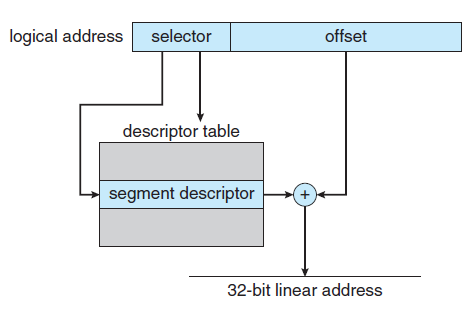
\includegraphics[scale=0.9]{os15.png}
    \caption{Segmentation hardware of Intel IA-32}
    \label{fig:my_label_15}
\end{figure}

\begin{figure}[!h]
    \centering
    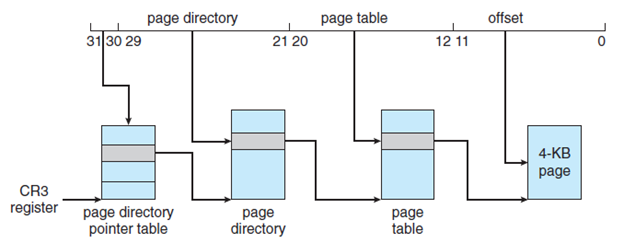
\includegraphics[scale=0.8]{os16.png}
    \caption{PAE in Intel IA-32}
    \label{fig:my_label_16}
\end{figure}

\subsection{Windows}
\begin{itemize}
    \item Windows uses demand paging in conjunction with \textbf{clustering} to implement virtual memory management. 
    
    \item In clustering, if a page fault occurs, then the pages that are close by to the faulted page (in a cluster) are all brought in (instead of only the faulted page). This takes advantage of the principle of locality. 
    
    \item When a process is created, it is assigned a \textbf{working set maximum} (largest possible number of pages in memory for that process) and a \textbf{working set minimum} (min number of pages that is guaranteed to have in memory for that process) . 
    
    \item If a process that is already at the working set maximum undergoes a page fault, local LRU replacement is used to load the new page. 
    
    \item If the amount of free memory falls below a threshold, then all processes undergo \textbf{automatic working set trimming}. For each process, if it has been allocated more pages than the working set minimum, the extra pages are removed. 
    
    \item Processes that are already at their working set minimum can be allocated some pages if available. 
    
    \item Windows performs working set trimming on user as well as system processes
\end{itemize}

\subsection{Solaris}
\begin{itemize}
    \item Solaris maintains a \texttt{lotsfree} variable that represents the threshold for number of free pages in memory. Normally it is set to 1/64 of total physical memory size. 
    
    \item If number of free frames falls below \texttt{lotsfree}, a process called \textbf{pageout} begins. A check for this is done 4 times per second. 
    
    \item The \textbf{reference bit} is a bit in the page table that is set every time that page is referenced in the process. 
    
    \item There are two scanners involved in the pageout process. The first scanner scans all the pages and sets the reference bit to 0 for all. The second scanner follows the first scanner and checks for all the pages that still have 0 reference bit (between the first and second scanners processes are still running and they might make references to some pages hence setting those bits to 1). 
    
    \item If the frame with reference bit 0 has been modified, then the second scanner also writes it to the disk. Then this frame is added to the free frame list. 
    
    \item The \texttt{scanrate} parameter is used to control the rate of scanning. When the amount of free memory falls below \texttt{lotsfree} then scanning starts at the rate of \texttt{slowscan}, progressing up to a maximum possible rate of \texttt{fastscan}. 
    
    \item The \texttt{handspread} parameter controls the distance between the two scanners (in terms of number of pages). 
    
    \item If free memory falls below the value of \texttt{desfree}, pageout will run a hundred times per second with the intention of keeping at least \texttt{desfree} free memory available.
    
    \item Enhancements to this algorithm in recent releases include ignoring shared pages for scanning, and giving priority to process files over normal memory files, also called \textbf{priority paging}. 
\end{itemize}

\begin{figure}[!h]
    \centering
    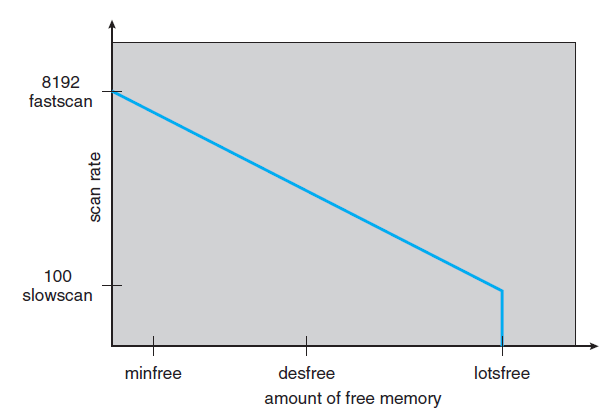
\includegraphics[scale=0.8]{os17.png}
    \caption{Solaris page scanning rate}
    \label{fig:my_label_17s}
\end{figure}
\end{document}